\section{Legislación}

Este proyecto ha sido desarrollado bajo los reglamentos y leyes marcados tanto por la Unión Europea como por el estado Español.

\subsection{Reglamento General de Protección de Datos - RGPD}
El RGPD~\cite{gdpr2016} es un conjunto de reglas aprobadas por el \textit{Parlamento Europeo} con el fín de proteger a las personas físicas en lo que corresponde al tratamiento y circulación de datos personales. Entre los artículos del RGPD que afectan a este proyecto, destacan:

\begin{itemize}
    \item \textbf{\textit{Capítulo II, Artículo 5}}, los datos necesarios para el registro de usuario han sido reducidos a los mínimos imprescindibles, siendo: nombre de usuario, descripción, correo y contraseña. El uso de esta información es meramente con fines de autenticación y distinción pública del usuario dentro de la aplicación web. Toda la información sobre el tratamiento de los datos está disponible en el aviso legal y los términos y condiciones del usuario.
    
    \item \textbf{\textit{Capítulo II, Artículo 6 y Artículo 7}}, el usuario dispondrá de acceso a los terminos y condiciones de la aplicaicón web, así como la posibilidad para aceptarlos manualmente. La aceptación implica que el usuario ha sido informado y accede al tratamiento de sus datos, además de aceptar la responsabilidad de cumplir con las normas de uso de la aplicación web. Los terminos y condiciones aceptados serán aquellos con publicación anterior a la fecha de creación de la cuenta de usuario.
    
    \item \textbf{\textit{Capítulo III, Artículo 12 y Artículo 13}}, el usuario dispondra en todo momento de información sobre: el tratamiento de datos de su cuenta de usuario, las normas de uso de la aplicación web y la identificación y contacto del responsable, todo a través del aviso legal y los términos y condiciones.
    
    \item \textbf{\textit{Capítulo III, Artículo 16}}, el usuario podrá modificar cualquier información publicada por si mismo en la aplicación web.

    \item \textbf{\textit{Capítulo III, Artículo 17}}, el usuario podrá eliminar su cuenta en cualquier momento, implicando la eliminación total de la información asociada a su cuenta.
    
    \item \textbf{\textit{Capítulo IV, Artículo 30}}, se redactó el \textit{Registro de las Actividades de Tratamiento} - RoPA~\figref{fig:registro_art30}.
    
    \begin{figure}[H]
        \centering
        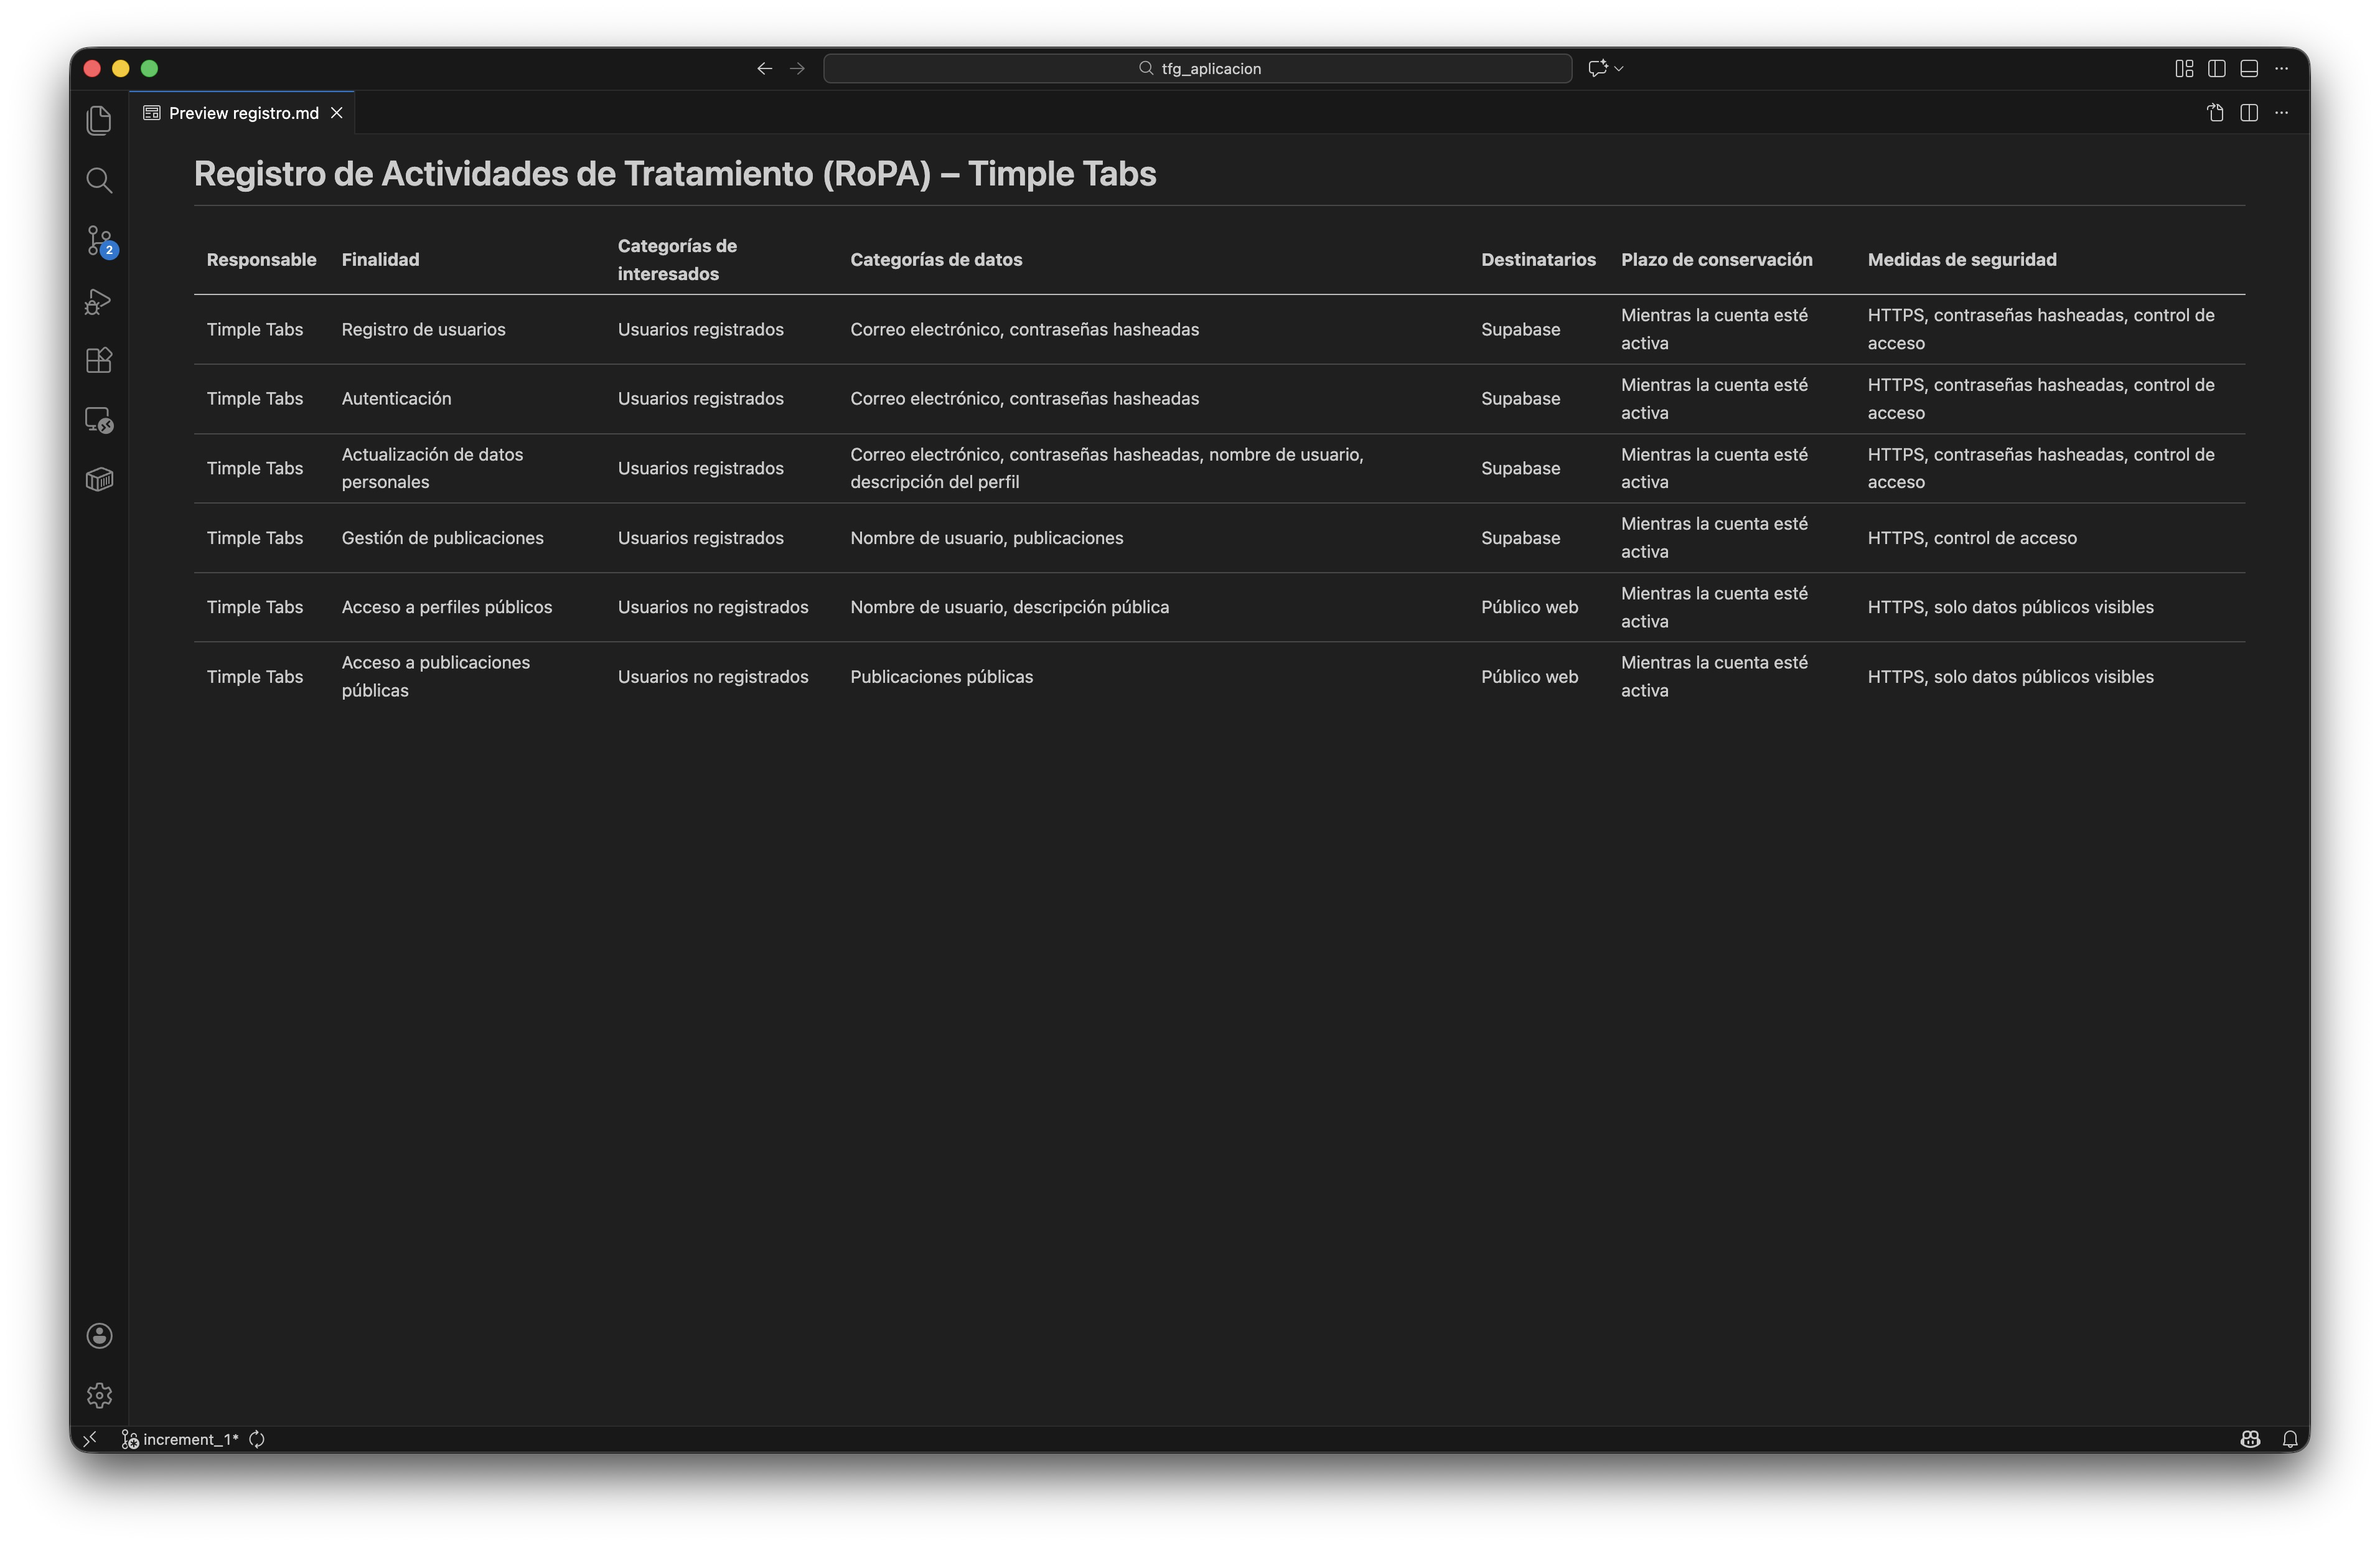
\includegraphics[width=0.8\textwidth]{Ilustraciones/normativa/registro_art30.jpeg}
        \caption{Fichero RoPA de Timple Tabs}\label{fig:registro_art30}
    \end{figure}
\end{itemize}

\subsection{Ley Orgánica de Protección de Datos y Garantía de Derechos Digitales - LOPDGDD}

La LOPDGDD~\cite{lopdgdd2018} es una ley orgánica aprobada en España por las \textit{Cortes Generales} que implementa las reglas descritas en el RGPD con el fín de adaptarlas al derecho interior y contexto del país. Con respecto a los artículos que afectan a este proyecto, excluyendo los ya mencionados en la RGPD, destaca el \textbf{\textit{Título 2, Artículo 7}} que tal y como recogen los terminos y condiciones de la aplicación web, no podrán registrarse menores de 14 años.